\begin{figure*}[t!]
\centering
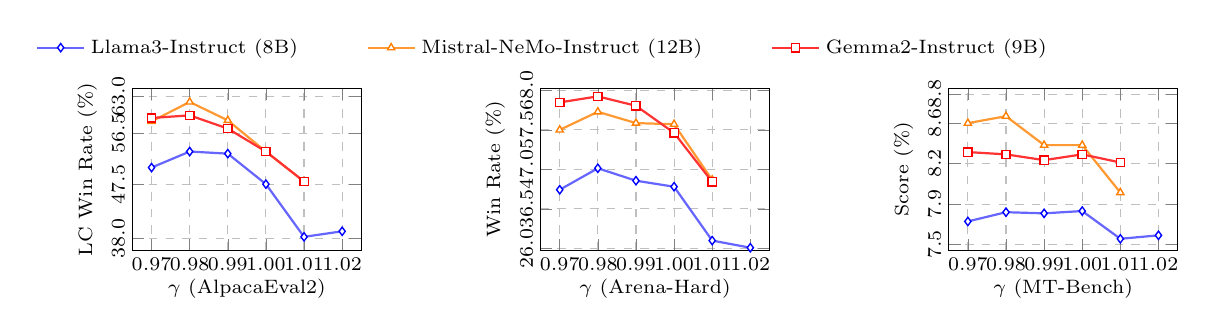
\begin{tikzpicture}
\scriptsize{
    \begin{axis}[
        at={(0,0)},
        height=.30\textwidth,
        width=.37\textwidth,
        ymajorgrids,
        xmajorgrids,
        grid style=dashed,
        xlabel={\scriptsize{$\gamma$} (AlpacaEval2)},
        ylabel={\scriptsize{LC Win Rate (\%)}},
        xtick={0.97, 0.98, 0.99, 1.00, 1.01, 1.02},
        ytick={38.0, 47.5, 56.5, 63.0},
        ylabel style={yshift=0em},
        xlabel style={yshift=0.3em, align=center},
        yticklabel style={/pgf/number format/fixed,/pgf/number format/fixed zerofill,/pgf/number format/precision=1, rotate=90},
        xticklabel style={/pgf/number format/fixed,/pgf/number format/fixed zerofill,/pgf/number format/precision=2},
        legend style={cells={align=left},
            draw=none,
            line width=1pt,
            at={(1.8,1.12)},
            anchor=south},
            legend columns=-1, /tikz/every even column/.append style={column sep=0.8cm}
            ]
        legend cell align={left},
        xtick align=inside,
        ymin=38.0, ymax=63.8,
        xmin=0.965, xmax=1.025,
        ]

        \addplot[blue!60,mark=diamond*,mark size=1.5pt,thick,mark options={fill=white,draw=blue,line width=0.5pt}] coordinates {(0.97,50.52) (0.98,53.34) (0.99,52.97) (1.00,47.60) (1.01,38.32) (1.02,39.30)};
        \node[red,mark=x,mark size=3pt,thick] at (axis cs:1.02,39.30) {};

        \addplot[orange!80,mark=triangle*,,mark size=1.5pt,thick,mark options={fill=white,draw=orange,line width=0.5pt}] coordinates 
        {(0.97,58.65) (0.98,62.07) (0.99,58.83) (1.00,53.32) (1.01,48.06)};
        \node[red,mark=x,mark size=3pt,thick] at (axis cs:1.02,0) {};
        
        \addplot[red!80,mark=square*,,mark size=1.5pt,thick,mark options={fill=white,draw=red,line width=0.5pt}] coordinates 
        {(0.97,59.25) (0.98,59.71) (0.99,57.38) (1.00,53.34) (1.01,48.06)};
        \node[red,mark=x,mark size=3pt,thick] at (axis cs:1.02,5) {};
        \legend{Llama3-Instruct (8B), Mistral-NeMo-Instruct (12B), Gemma2-Instruct (9B)}
        % \addlegendentry{Llama3-Instruct (8B)};
        % \addlegendentry{Mistral-NeMo-Instruct (12B)};
        % \addlegendentry{Gemma2-Instruct (9B)};
    \end{axis}
    }

\scriptsize{
    \begin{axis}[
        at={(18.5em,0)},
        height=.30\textwidth,
        width=.37\textwidth,
        ymajorgrids,
        xmajorgrids,
        grid style=dashed,
        xlabel={\scriptsize{$\gamma$} (Arena-Hard)},
        ylabel={\scriptsize{Win Rate (\%)}},
        xtick={0.97, 0.98, 0.99, 1.00, 1.01, 1.02},
        ytick={26.0, 36.5, 47.0, 57.5, 68.0},
        ylabel style={yshift=0em},
        xlabel style={yshift=0.3em, align=center},
        yticklabel style={/pgf/number format/fixed,/pgf/number format/fixed zerofill,/pgf/number format/precision=1, rotate=90},
        xticklabel style={/pgf/number format/fixed,/pgf/number format/fixed zerofill,/pgf/number format/precision=2},
        legend style={at={(0.01,0.0)}, anchor=south, draw=none, line width=1pt, legend columns=-1},
        legend cell align={left},
        xtick align=inside,
        ymin=25.5, ymax=68.5,
        xmin=0.965, xmax=1.025,
        ]

        \addplot[blue!60,mark=diamond*,mark size=1.5pt,thick,mark options={fill=white,draw=blue,line width=0.5pt}] coordinates {(0.97,41.6) (0.98,47.3) (0.99,44.0) (1.00,42.4) (1.01,28.1) (1.02,26.2)};

        \addplot[orange!80,mark=triangle*,,mark size=1.5pt,thick,mark options={fill=white,draw=orange,line width=0.5pt}] coordinates {(0.97,57.5) (0.98,62.3) (0.99,59.3) (1.00,59.0) (1.01,44.2)};

        \addplot[red!80,mark=square*,,mark size=1.5pt,thick,mark options={fill=white,draw=red,line width=0.5pt}] coordinates {(0.97,64.8) (0.98,66.4) (0.99,63.9) (1.00,56.7) (1.01,43.7)};

    \end{axis}
    }

\scriptsize{
    \begin{axis}[
    at={(37em,0)},
        height=.30\textwidth,
        width=.37\textwidth,
        ymajorgrids,
        xmajorgrids,
        grid style=dashed,
        xlabel={\scriptsize{$\gamma$} (MT-Bench)},
        ylabel={\scriptsize{Score (\%)}},
        xtick={0.97, 0.98, 0.99, 1.00, 1.01, 1.02},
        ytick={7.50, 7.85, 8.20, 8.55, 8.80},
        ylabel style={yshift=0em},
        xlabel style={yshift=0.3em, align=center},
        yticklabel style={/pgf/number format/fixed,/pgf/number format/fixed zerofill,/pgf/number format/precision=1, rotate=90},
        xticklabel style={/pgf/number format/fixed,/pgf/number format/fixed zerofill,/pgf/number format/precision=2},
        legend style={at={(0.01,0.0)}, anchor=south, draw=none, line width=1pt, legend columns=-1},
        legend cell align={left},
        xtick align=inside,
        ymin=7.45, ymax=8.85,
        xmin=0.965, xmax=1.025,
        ]

        \addplot[blue!60,mark=diamond*,mark size=1.5pt,thick,mark options={fill=white,draw=blue,line width=0.5pt}] coordinates {(0.97,7.7) (0.98,7.78) (0.99,7.77) (1.00,7.79) (1.01,7.55) (1.02,7.58)};

        \addplot[orange!80,mark=triangle*,,mark size=1.5pt,thick,mark options={fill=white,draw=orange,line width=0.5pt}] coordinates {(0.97,8.55) (0.98,8.61) (0.99,8.36) (1.00,8.36) (1.01,7.95)};

        \addplot[red!80,mark=square*,,mark size=1.5pt,thick,mark options={fill=white,draw=red,line width=0.5pt}] coordinates {(0.97,8.30) (0.98,8.28) (0.99,8.23) (1.00,8.28) (1.01,8.21)};
        \node[red,mark=x,mark size=3pt,thick] at (axis cs:1.02,1.5) {};
    \end{axis}
    }
\end{tikzpicture}
\caption{Performance against different $\gamma$ choices of three open-source models on three benchmarks.}
\label{fig:gamma_vs_winrate}
\end{figure*}
